\begin{frame}
  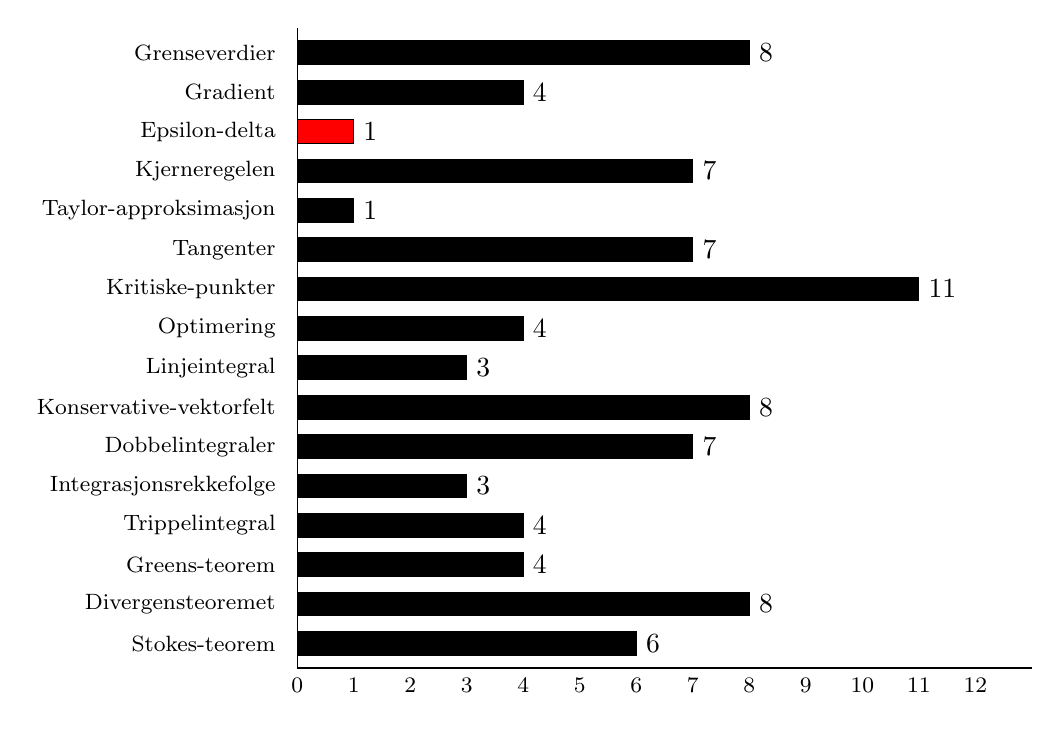
\begin{tikzpicture}
    \begin{axis}[ xbar=0pt, /pgf/bar shift=0pt, legend style={ legend columns=4,
        at={(xticklabel cs:0.5)}, anchor=north, draw=none }, ytick={0,...,15},
      ytick style={draw=none},% <- added
      axis y line*=none, axis x line*=bottom, tick label
      style={font=\footnotesize}, legend style={font=\footnotesize}, label
      style={font=\footnotesize}, xtick style={draw=none},% <- added
      xtick={0,1,...,12}, width=.9\textwidth, bar width=3mm, y dir = reverse,
      xmin=0, xmax=13, area legend,
      y=5mm, enlarge y limits={abs=0.625},
      style={text=black}, every axis plot/.append style={fill},
      nodes near coords, nodes near coords,
      yticklabels={%
        {\topicref{Grenseverdier}},
        {\topicref{Gradient}},
        {\topicref{Epsilon-delta}},
        {\topicref{Kjerneregelen}},
        {\topicref{Taylor-approksimasjon}},
        {\topicref{Tangenter}},
        {\topicref{Kritiske-punkter}},
        {\topicref{Optimering}},
        {\topicref{Linjeintegral}},
        {\topicref{Konservative-vektorfelt}},
        {\topicref{Dobbelintegraler}},
        {\topicref{Integrasjonsrekkefolge}},
        {\topicref{Trippelintegral}},
        {\topicref{Greens-teorem}},
        {\topicref{Divergensteoremet}},
        {\topicref{Stokes-teorem}}}]
      \addplot[fill=black] coordinates {(8,0)};
      \addplot[fill=black] coordinates {(4,1)};
      \addplot[fill=red] coordinates {(1,2)};
      \addplot[fill=black] coordinates {(7,3)};
      \addplot[fill=black] coordinates {(1,4)};
      \addplot[fill=black] coordinates {(7,5)};
      \addplot[fill=black] coordinates {(11,6)};
      \addplot[fill=black] coordinates {(4,7)};
      \addplot[fill=black] coordinates {(3,8)};
      \addplot[fill=black] coordinates {(8,9)};
      \addplot[fill=black] coordinates {(7,10)};
      \addplot[fill=black] coordinates {(3,11)};
      \addplot[fill=black] coordinates {(4,12)};
      \addplot[fill=black] coordinates {(4,13)};
      \addplot[fill=black] coordinates {(8,14)};
      \addplot[fill=black] coordinates {(6,15)};
    \end{axis}
  \end{tikzpicture}
\end{frame}

\begin{frame}
  \subsection{Epsilon-Delta}\label{subsec:Epsilon-delta}
  \frametitle{Epsilon-Delta}\centerline{
  \only<1>{\includegraphics[scale=0.95]{../img/epsilon-delta}}%
  \only<2>{\includegraphics[scale=0.95]{../img/epsilon-delta-1}}
  \only<3>{\includegraphics[scale=0.95]{../img/epsilon-delta-2}}
  \only<4>{\includegraphics[scale=0.95]{../img/epsilon-delta-3}}}
[Vi sier at $f$ er \emph{kontinuerlig} i $\A$ dersom det for \only<1-3>{alle}<4>{\emph{alle}} $\varepsilon >
0$ eksisterer en $\delta > 0$ slik at
%
$
  \norm{f(\X) - f(\A)} < \varepsilon$ når $\norm{\X - \A} < \delta
  $.]\\
  Intuisjon: uansett hvor nærme vi er $\A$ kan vi alltid komme \emph{litt} nærmere.
\end{frame}

\begin{frame}
  \frametitle{Epsilon-Delta}
  \begin{itemize}
    \item Kladd: Forenkle $\norm{f(\X) - f(\Y)}$ til du oppnår ulikheten
      $\norm{f(\X)-f(\Y)} \leq K \norm{\X - \Y}$.
    \item Bevis: Skriv opp definisjonen ``ønsker å vise at for alle
      $\varepsilon>0$ eksisterer det en $\delta>0$ slik at''
      \begin{equation*}
    \norm{\X - \Y} < \delta \ \Longrightarrow \ \norm{f(\X) - f(\Y)} < \varepsilon.
  \end{equation*}
    \item Bevis: Velg $\delta = \varepsilon/K$. Da er
      \begin{align*}
        \norm{f(\X) - f(\Y)} \leq K \norm{\X - \Y} < K \delta \leq K(\varepsilon/K) = \varepsilon
      \end{align*}
    \item Litt som induksjon vi antar at $\norm{\X-\Y}<\delta$ stemmer (induksjonshypotesen).
  \end{itemize}
\end{frame}

\begin{frame}
  \begin{oppgave}{V2014, Oppgave 8}
    La funksjonen $f\colon A\subset \R^n \to \R^m$ oppfylle
    %
    $
      \norm{f(\X) - f(\Y)} \leq K \norm{\X - \Y}^{\alpha}
    $
    %
    for alle $x$, $y$ i $A$ hvor $K$ og $\alpha$ er positive. Vis at $f$ er en
    kontinuerlig funksjon.
  \end{oppgave}

\only<2>{\textbf{Kladd:} Antagelsen er at $\norm{\X - \Y}<\delta$. Slik at
%
\begin{equation*}
  \norm{f(\X) - f(\Y)}
  \leq K \norm{\X - \Y}^{\alpha}
  < K \delta^{\alpha}
\end{equation*}}
%
\visible<3->{%
\begin{proof}
  \visible<3->{Ønsker å vise at $f$ er kontinuerlig, med andre ord ønsker å vise at for alle
  $\varepsilon>0$ eksisterer det en $\delta>0$ slik at
  %
  \begin{equation*}
    \norm{\X - \Y} < \delta \ \Longrightarrow \ \norm{f(\X) - f(\Y)} < \varepsilon.
  \end{equation*}}%
%
\visible<4->{
  Velg $\delta = (\varepsilon/K)^{1/\alpha}$ da er
  %
  \begin{align*}
  \norm{f(\X) - f(\Y)}
    \leq K \norm{\X - \Y}^{\alpha}
    \visible<5->{%
    < K \delta^{\alpha}}
    \visible<6->{
    = K \left( \frac{\varepsilon^{1/\alpha}}{K^{1/\alpha}} \right)^{\alpha}
    = \varepsilon}
  \end{align*}}
  %
\visible<6->{som var det vi ønsket å vise.}
\end{proof}%
}
\end{frame}


%%% Local Variables:
%%% mode: latex
%%% TeX-master: "main"
%%% End:
